\chapter{Incidencias}

\section{Visión general}

	Como es normal, a lo largo del proyecto han surgido diferentes incidencias que han retrasado el proyecto o han hecho que el alcance o los requisitos del mismo hayan tenido que ser modificados. A continuación se muestran los problemas más relevantes y cómo se han solucionado.

\section{Conversión de XML a JSON}

	Como ya se ha explicado, se decidió utilizar \acrshort{json} en el proyecto en vez de \acrshort{xml} por ser más conveniente. Sin embargo, no existe o no se ha encontrado ninguna herramienta que generase archivos con coordenadas gráficas y animaciones en \acrshort{json}, pero existen muchas que crean archivos \acrshort{xml}, así que se decidió que se traducirían. Hacerlo a mano no era viable, ya que llevarían demasiado tiempo y existían muchas posibilidades de cometer errores. La segunda opción consistía en crear un pequeño que recibiese un \acrshort{xml} y lo tradujese a \acrshort{json}, pero de nuevo esta opción no era conveniente por los mismos problemas, además de que la complejidad del algoritmo sería grande. Por tanto se decidió buscar una herramienta que los convirtiese, y tras barajar unas cuantas posibilidades se decidió usar el servicio web XML to JSON.

	XML to JSON cumplió su cometido, pero también introdujo nuevos problemas. En \acrshort{json}, los valores de cada par clave-valor pueden ser de distintos tipos: cadenas, números, objetos, matrices, valores booleanos o valor nulo. La aplicación web citada convertía adecuadamente los valores del \acrshort{xml} a \acrshort{json}, todos excepto uno. Por alguna razón, el conversor en vez de escribir valores numéricos, escribía cadenas que contenían el número. Esto conllevó que el algoritmo hecho para analizar los \acrshort{json} y crear las animaciones fallaba, ya que esperaba encontrar números y encontraba cadenas. Por suerte, la solución fue bastante sencilla: simplemente se leyeron los valores como cadenas y, utilizando funciones de la librería estándar de C++, se convirtieron a números antes de ser usadas. A pesar de que esta solución hace que el algoritmo sea algo más lento, se consideró la solución más apropiada, ya que la aplicación de la misma era muy sencilla y el coste temporal mínimo.

	\begin{figure}[!htp]
		 \centering
		 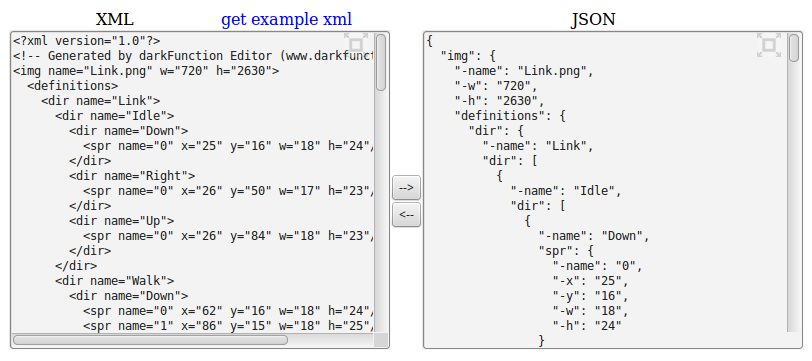
\includegraphics[scale=.5]{fig/conversionNums}
		 \caption{Ejemplo del error de conversión de números}
		 \label{fig:conversionNums}
	\end{figure}

	\FloatBarrier

\section{SFML del repositorio desactualizada}

	\acrshort{tgui}, la librería utilizada para crear las interfaces gráficas de usuario, es muy estricta con las versiones de \acrshort{sfml} con las que trabaja. Cada versión exige una versión de \acrshort{sfml} y solo ofrece compatibilidad con versiones posteriores, nunca retrocompatibilidad. En el momento en el que instaló por primera vez la entonces última versión de \acrshort{tgui}, esta requería utilizar la versión 2.2 de \acrshort{sfml}, que también era en ese momento la última disponible. Dado que \acrshort{sfml} se instaló desde el repositorio oficial, se asumió que se habría instalado dicha versión, pero no fue así. Por algún motivo, el repositorio aún servía la versión anterior, la 2.1, de forma que al intentar utilizar la librería \acrshort{tgui} aparecían un montón de errores y la aplicación no funcionaba. En este punto había dos opciones: utilizar una versión más antigua de \acrshort{tgui} que fuese compatible con \acrshort{sfml} 2.1 o actualizar \acrshort{sfml} a la versión 2.2. Se decidió actualizar \acrshort{sfml}, ya que la nueva versión corregía algunos errores y traía mejoras en la funcionalidad, lo que ayudaría a conseguir un producto final más robusto.

\section{Error de inicialización de palanca de juego}

	En un punto del proyecto, sin razón aparente, apareció repentinamente el siguiente error al ejecutar el juego:

	\begin{figure}[!htp]
		 \centering
		 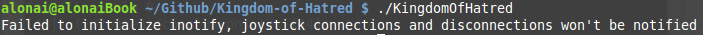
\includegraphics[scale=.5]{fig/inotify}
		 \caption{Captura del error de inicialización}
		 \label{fig:inotify}
	\end{figure}

	\FloatBarrier

	Aparentemente, el error se da debido a que \acrshort{sfml} no detecta adecuadamente las palancas de control. Cabe mencionar que, aunque \acrshort{sfml} provea soporte para palancas de control y mandos, no se han utilizado en el proyecto en ningún momento, de forma que no debería haber errores a causa de ello. Sin embargo, \acrshort{sfml} siempre inicializa el módulo encargado de ello, y en ocasiones falla. Se investigó sobre el problema y se vió que ya había sido reportado por varios usuarios desde la versión 2.1 de \acrshort{sfml}, y al parecer ocurría en sistemas que utilizaban un sistema operativo basado en Ubuntu cuando había muchos archivos abiertos. Asumiendo esto, el error debería desaparecer si se cerraban archivos, pero no era así. El error persistía y no desaparecía a pesar de que se reiniciara el ordenador o se recompilase el programa. Finalmente, la forma de solucionarlo fue la siguiente: se desintalaron tanto \acrshort{sfml} como \acrshort{tgui} y se reinstalaron en sus versiones más recientes. Durante el desarrollo del proyecto la versión 2.3 \acrshort{sfml} fue lanzada, y \acrshort{tgui} se actualizó también con una versión compatible con \acrshort{sfml} 2.3. Se procedió a reinstalar ambas librerías y, al recompilar el código, el error desapareció.
